\section{Predicate Exchange}

% Predicate exchange is /a procedure to sample from a model conditioned on a predicate.
% To condition a model on a predicate we develop \emph{predicate exchange}, a likelihood-free inference procedure. 
Given a model (a collection of random variables)  $\vect{X} = (X_1, X_2, \dots, X_n)$ and a predicate $\lk$ which maps a model realization  $\vect{x} = (x_1, x_2, \dots, x_n)$ to 0 or 1, predicate exchange samples from the posterior distribution of $\vect{X}$ conditioned on $\ell$ through two steps:
\begin{enumerate}
\item \textbf{Predicate Relaxation} constructs a soft predicate $\soft{\lk}$ from $\lk$. $\soft{\lk}$ takes values in a continuous Boolean algebra: the unit interval $[0, 1]$ with continuous logical connectives $\soft{\land}$, $\soft{\lor}$ and $\neg$.
$\soft{\lk}$ is 1 iff $\lk$ is 1, but otherwise takes nonzero values denoting the degree to which $\lk$ is satisfied.
% The relaxation is parameterized by a temperature.
% Predicate relaxation allows us to apply likelihood based MCMC inference procedures.
\item  \textbf{Replica Exchange} is a Markov Chain Monte Carlo procedure that simulates several replicas of $\soft{\lk}$ in parallel. 
\end{enumerate}

In this section we formalize the construction of $\soft{\lk}$ from $\lk$, and sampling from models conditioned on $\soft{\lk}$.

\subsection{Predicate Relaxation}\label{predexchange}

Our objective is to construct a soft predicate $\soft{\lk}$ that introduces approximations into $\lk$ to make inference more tractable.
We refer to $\soft{\lk}$ as a \emph{relaxation} of $\lk$.
Informally, these approximations mean that while conditioning on $\lk$ eliminates a set of possible values, conditioning on $\soft{\lk}$ only makes them less likely.
% Formally, $\soft{Y}$ approximates
% the sense that \todo{IN WHICH WAY?}when viewed as a likelihood function on model parameters, $\soft{\lk}$ has a broader support, assigning nonzero weights to parameter values which have zero weight under $\lk$.

A relaxation $\soft{\lk}$ has a temperature parameter $\alpha$ that controls the fidelity of the approximation.
There are three desiderata which govern this approximation.
In particular, $\soft{\lk}$ should (i) converge to $\lk$ as $\alpha \to 0$, (ii) converge to 1 as $\alpha \to \infty$, and (iii) be consistent with $\lk$ on 1, i.e., $\lk(\vect{x}) = 1$ iff $\softv{\lk}(\vect{x}) = 1$ at all temperatures.  
Formally:

% The family of approximations of the predicate $Y$ is parameterized through a temperature $\alpha$ that controls the smoothness of the approximation. In particular, $\soft{\lk}$ with $\alpha \to 0$ converges to $Y$ itself while increasing values of $\alpha$ yield smoother approximations eventually giving a flat surface when $\alpha \to \infty$. Moreover, the set of conditional samples $C(Y) = \{ \omega \in \Omega \text{ } | \text{ } Y(\omega) = 1 \}$ are assigned a value of $1$ in $\soft{\lk}$ for all temperatures. 

% To construct a $\soft{\lk}$ with such properties, we let $Y$ be the following predicate $a=b$ for standard Gaussians $a, b \sim \mathcal{N}(0, 1)$. We choose a distance
% $\rho(a, b)$ to indicate how close our sample is to $C(Y)$. To meet the desiderata
% of having $C(Y)$ be $1$ over the constraint set and to ensure the constraint becomes
% smoother with large $\alpha$, we use a function $k : [0, \infty] \to [0, 1]$ parameterized by $\alpha$ to wrap the distance $\rho(a, b)$. A simple choice for such a function is $k(d; \alpha) = e^{-d / \alpha}$ that provides the desired properties to $\soft{\lk}$ (see Appendix). The formal definition of $\soft{\lk}$ is as follows.

\begin{definition}
$\softv{\lk} : \xp \to [0, 1]$ parameterized by $\alpha \in [0, \infty)$ is a relaxation of $\lk: \xp \to \{0, 1\}$ if for all $\vect{x} \in \xp$:
\begin{enumerate}[label=(\roman*)]
	\label{def:temp}
	\item $\lim_{\alpha \to 0}\softv{\lk}(\vect{x}; \alpha) = \lk(\vect{x})$.
	\item $\lim_{\alpha \to \infty}\softv{\lk}(\vect{x}; \alpha) = 1$.
  \item for all $\alpha < \infty$, $\softv{\lk}(\vect{x}; \alpha) = 1$ iff $\lk(\vect{x}) = 1$.
\end{enumerate}
\end{definition}

\todo{Explain motivate each of these desiderata}

\paragraph{Distance Based Satisfiability}
To construct $\soft{\lk}$ we assume $\xp$ has a metric, and define $\softv{\lk}(\vect{x})$ -- the degree to which $\vect{x}$ satisfies $\lk$ -- as the \emph{distance} from $\vect{x}$ to an element in $\xp$ that satisfies $\ell$.
In general there are several values which satisfy $\ell$ and several corresponding distances.
Naturally, we are interested in the smallest distance, since it indicates the smallest change we could make to $\vect{x}$ to satisfy $\lk$.
With respect to a metric $\rho$, we refer to the soft predicate that maps $\vect{x}$ to its distance to the closest satisfying element in $\xp$ as the \emph{tightest} relaxation of $\ell$:

\begin{definition}
Let $\rho$ be a metric on $\xp$, $k_\alpha$ be a relaxation kernel (described below) which bounds distances to $[0, 1]$, and $A = \{\vect{x} \mid \lk(\vect{x}) = 1\}$ be the satisfying set.
The predicate $\softv{\lk}_{\inf}(\vect{x})$ is the tightest relaxation of $\ell$ and defined as:
\begin{equation}\label{eq;linf}
\softv{\lk}_{\inf}(\vect{x}) = k_\alpha(\rho(\vect{x}, A))
\end{equation}
The distance $\rho(\vect{x}, A) = \inf \left\{\rho(\vect{x}, a) \mid a \in A\right\}$ is the smallest distance between $\vect{x}$ and any element of $A$.
% As shown in the Section \ref{implement}, $\soft{\lk}_{\inf}$ can be difficult to compute.
\end{definition}

\paragraph{Product Metrics}The metric $\rho$ is parameterized by the type of input.
For canonical spaces such as $\mathbb{R}$ and $\mathbb{N}$ we default to the Euclidean distance. 
We can construct $\rho$ automatically for composite elements $x, y \in \mathbb{T}_1 \times \cdots \times \mathbb{T}_n$ of product types, by taking the mean of distances of components: $\rho(x, y) = (1/n)\sum^n_{i=1}\rho(x_i, y_i)$.

% $$
% d_{p}((x_{1},\ldots ,x_{n}),(y_{1},\ldots ,y_{n}))=\|\left(d_{X_{1}}(x_{1},y_{1}),\ldots ,d_{X_{n}}(x_{n},y_{n})\right)\|_{p}}
% $$

\paragraph{Relaxation Kernels} A relaxation kernel $k_\alpha$ bounds distances from $\mathbb{R}$ to the unit interval, and is paramterized by temperature $\alpha$.
A relaxation kernel is valid if soft-predicates constructed with it satisfy the aforementioned relaxation axioms.
One such kernel, which we restrict our attention to, is the squared exponential kernel:
\begin{equation}
k_{\alpha}(r) = \exp\left(-\frac{r^2}{\alpha}\right)
\end{equation}




  % \begin{center}
  % \begin{tabular}{ c |  c | c }
  %   \hline		
  %   $x \soft{=} y$ & $x \soft{>} y$ & $x \soft{<} y$  \\
  %   $k_\alpha(\rho(x, y))$ & $k_\alpha(\rho(x, [y, \infty]))$ & $k_\alpha(\rho(x, [-\infty, y]))$ \\
  %   \hline  
  % \end{tabular}
  % \end{center}



\paragraph{Soft Primitives}
To soften complex programs we first define relaxations for numerical and logical primitives.
Soft equality is straightforward: $x \soft{=} y$ is defined as $k_\alpha(\rho(x, y))$.
A soft inequality such as $x \soft{>} y$ is a function of the amount by which $x$ must be increased (or $y$ decreased) until $x > y$ is true.
This is the distance between $x$ and the interval $[y, \infty]$, where the distance between a point and any interval $[a, b]$ is the smallest distance between $x$ and any element in $[a, b]$, and therefore 0 if $x \in [a, b]$:
\begin{equation}
\rho(x, [a, b]) =
\begin{cases}
  a - x & \text{ if } x < a\\
  x - b & \text{ if } x > b\\
  0              & \text{otherwise}
\end{cases}
\end{equation}
Soft conjunction $\soft{\land}$ and disjunction $\soft{\lor}$ take the $\min$ and $\max$ respectively, which is standard.
Soft negation, on the other hand, introduces complications.
In continuous logics \cite{kimmig2012short}, the negation of $a \in [0, 1]$ is $1 - a$.
However, as shown in Figure \ref{negationimg} (b), this violates criteria (iii) of predicate relaxation; there are values which satisfy the hard predicate $\neg(x > 0)$ which do take a value of 1 in $1 - (x \soft{>} 0)$.
Figure \ref{negationimg} illustrates this issue.


\begin{figure}
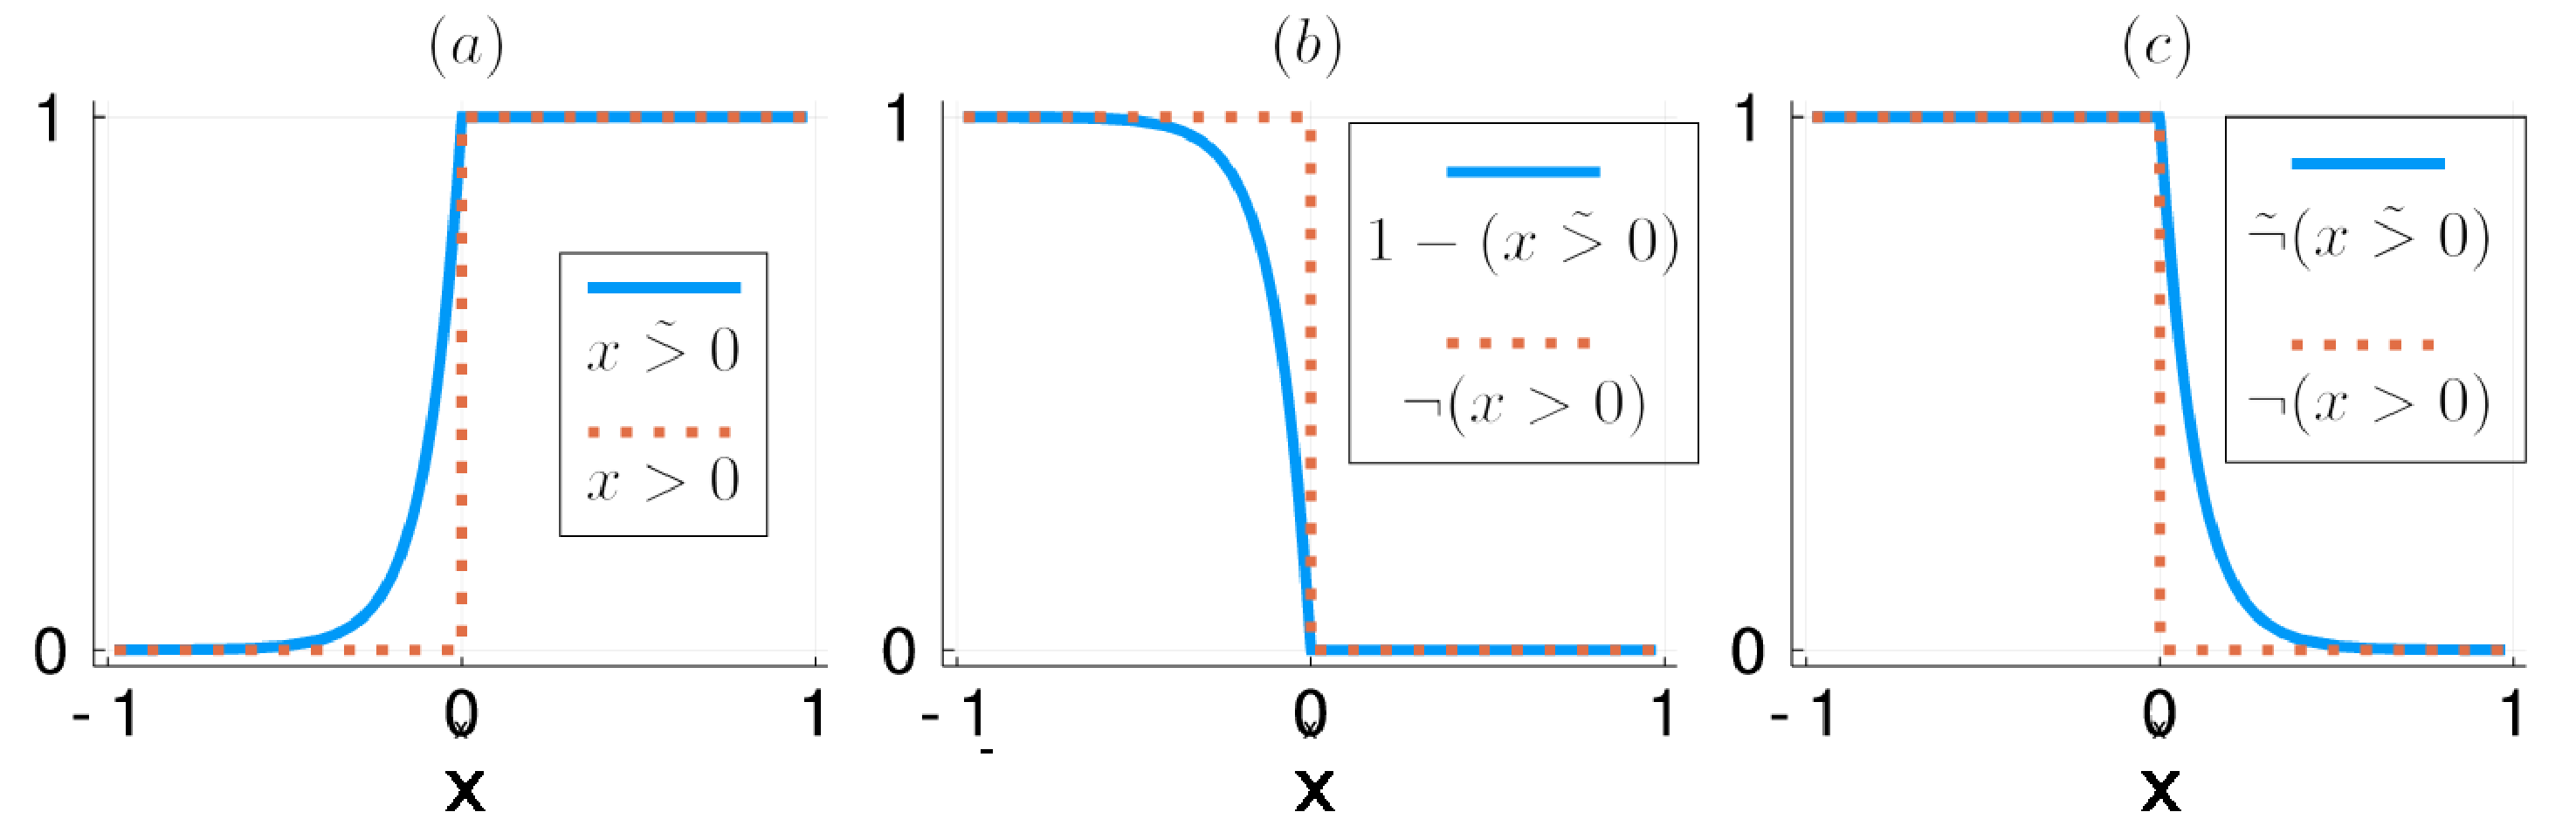
\includegraphics[width=\linewidth]{negation.eps}
\caption{The problem of negation.  In all figures, soft (blue) and hard (red, dashed) predicates as a function of $x$.  Left: $x \soft{>} y$ approximates $x > y$. Middle:  the standard approach to continuous negation $(1- (x \soft{>} y))$ violates relaxation criteria (iii). Right: the desired outcome of soft negation of $x \soft{>} y$.}\label{negationimg}
\end{figure}


The problem of negation arises because $\soft{\lk}$ is consistent with $\lk$ at 1 but not at 0, i.e., $\softv{\lk}(\vect{x}; \alpha) = 1$ iff $\lk(\vect{x}) = 1$ at all temperatures $\alpha$.
In other words, $\soft{\lk}$ is a one-sided approximation.
To resolve this, \emph{two-sided} soft primitives yield a pair $(a_0, a_1)$ where $a_0, a_0 \in [0, 1]$.
$a_1$ is consistent with $\lk$ on $1$, just as before, while $a_0$ is consistent with $\neg \lk$ on $1$.
For example if $x \dsoft{>} 0$ returns $(a_0, a_1)$, then as a function of $x$, $a_1$ is 1 iff $x > 0$ (Figure \ref{negationimg} (a)) and $a_0$ is 1 iff $x \leq 0$ (Figure \ref{negationimg} (c)).
Two-sided soft conjunction and soft disjunction follow De Morgan's laws.
Soft negation then simply swaps the elements of $(a_0, a_1)$ to yield $(a_1, a_0)$.
A complete two-sided soft logic is shown in Figure \ref{softw}.

As an operation, conditioning does not treat 0 and 1 outputs of a predicate symmetrically.
Rather, it restricts the model to values which produce 1.
Consequently, we define conditioning on a $(a_0, a_1)$ as conditioning on only $a_1$.

% \begin{definition}
% The function $\softv{Y} : \Omega \to [0, 1]^2$ parameterized by $\alpha \in [0, \infty)$ is a two-sided relaxation of a $Y: \Omega \to \{0, 1\}$ if:
% \begin{enumerate}[label=(\roman*)]
% 	\label{def:temp}
% 	\item For all $\omega \in \Omega$, $\lim_{\alpha \to 0}\softv{Y}(\omega; \alpha) = (\neg Y(\omega), Y(\omega))$.
% 	\item For all $\omega \in \Omega$, $\lim_{\alpha \to \infty}\softv{Y}(\omega; \alpha) = (0, 1)$.

%     \item For all $\alpha$, $\softv{Y}(\omega; \alpha) = 1$ iff $Y(\omega) = 1$.
%     \item The entropy $H(\softv{Y}(\omega; \alpha))$ (which characterizes the fidelity of the approximation ) is an increasing function of $\alpha$.\footnote
%     {By compactness, it is integrable for all $\alpha$, when $\Omega$ has finite dimension}
% \end{enumerate}
% \end{definition}


\begin{figure}
\begin{align*}
x \dsoft{=} y &= (\text{if } x = y  \text{ then } \exp(-1/\alpha) \text{ else } 1, k_\alpha(\rho(x, y)))\\
x \dsoft{>} y &= (k_\alpha(\rho(x, [-\infty, y])), k_\alpha(\rho(x, [y, \infty])))\\
x \dsoft{<} y &= (k_\alpha(\rho(y, [x, \infty])), k_\alpha(\rho(y, [-\infty, x])))\\
(a_0, a_1) \dsoft{\land} (b_0, b_1) &= (\max(a_0, b_0), \min(a_1, b_1))\\
(a_0, a_1) \dsoft{\lor} (b_0, b_1) &= (\min(a_0, b_0), \max(a_1, b_1))\\
\softv{\neg}(a_0, a_1) &= (a_1, a_0)
\end{align*}
\caption{Two-sided soft primitive predicates}
\label{softw}
\end{figure}

% \begin{center}
% \begin{tabular}{ l | c | r }
%   % \hline		
%   $(a_0, a_1) \soft{\land} (b_0, b_1)$ & $(a_0, a_1) \soft{\lor} (b_0, b_1)$ & $\neg(a_0, a_1)$ \\
%   $(a_0, a_1) \soft{\land} (b_0, b_1)$ & $(a_0, a_1) \soft{\lor} (b_0, b_1)$ & $\neg(a_0, a_1)$ \\
%   % \hline  
% \end{tabular}
% \end{center}

\paragraph{Composition of Soft Primitives} We can construct $\soft{\lk}$ from $\lk$ compositionally, by substituting primitive predicates (equality, inequalities and logical operators) with soft counterparts.
% Here we describe the relaxation of predicates defined as compositions of primitive functions, and in section \ref{} we provide an implementation amenable to programs.
For instance the predicate $(x > y) \lor \neg(x^2 = 2)$ is relaxed by $(x \soft{>} y) \soft{\lor} \softv{\neg}(x^2 \soft{=} 2)$.
% In general, we use $\soft{p}$ to denote a relaxation of a predicate $p$.

\begin{proposition}Relaxation criteria are preserved under composition.
Let $a$ and $b$ be predicates, and $\circ$ denote a binary logical operator.  If $\softv{a}, \softv{b}$ and $\soft{\circ}$ are respective valid relaxations.  Then $\softv{a} \soft{\circ} \softv{b}$ is a relaxation of $a \circ b$.
\end{proposition}
% \emph{proof} Prove it.



\subsection{Approximate Markov Chain Monte Carlo}
We use soft predicates as approximate likelihoods, and as a result is amenable to likelihood based inference methods such as Markov Chain Monte Carlo.
MCMC algorithms require a function $f$ that is proportional to the the target density.
In Bayesian inference this is the posterior, dictated by Bayes' theorem as the product of the likelihood and the prior.
Approximate inference using soft predicates takes a similar form.

\begin{definition}
Let $\vect{X} = (X_1, \dots, X_n)$ be a model, $\lk$ be a predicate that conditions $\vect{X}$, and  $\vect{x}$ be a realization of $\vect{X}$.
Assuming a prior density $p$, the approximate posterior $f$ is the product:
\begin{equation}\label{fpm}
f(\vect{x}) = p(\vect{x}) \cdot \softv{\lk}(\vect{x})
  \end{equation}
\end{definition}
$\soft{\lk}$ down weights parameter values which violate $\lk$ by the degree to which they violate it. 
This is modulated by the temperature $\alpha$ used in the  relaxation kernels which constitute $\soft{\lk}$.
At maximum temperature $\soft{\lk}$ has no effect, and the approximate posterior $f$ is equal to the prior $p$.
At zero temperature, $f$ recovers the true posterior since parameter values which violate the condition are given zero weight.

For illustration, let $\vect{X} = (X_1, X_2)$ be a model where $X_{1,2} \sim \mathcal{N}(0, 1)$.
If the model is conditioned on $X_1 + X_2 = 0$, the approximate posterior is:
\begin{equation}\label{approxposterior}
f_\alpha(x_1, x_2) = \mathcal{N}_{0,1}(x_1) \cdot \mathcal{N}_{0,1}(x_2) \cdot k_\alpha(\rho(x_1 + x_2, 0)) 
\end{equation}

%  q
The temperature parameter trades off between tractability of inference and the fidelity of the approximation.
If the temperature is too high $\soft{\lk}$ will diverge too greatly from $\lk$. If it is too low, convergence will be slow.

\paragraph{Balancing Different Constraints}
At a fixed, nonzero temperature, the scales of variables affects their influence on
the conditional distribution.
For instance, consider two uniformly distributed random variables $x \sim \unif(-1, 1)$ and $y \sim \unif(-10, 10)$,
and predicates $p_x$, $p_y$ defined as $x \soft{=} 0$ and $y \soft{=} 0$ respectively.
The expectation of a soft predicate quantifies the degree to which it is true, and is a non-decreasing function of temperature.
The prior expectation of $p_x$ is significantly larger than that of $p_y$.
because values far from the 0 are more likely under $y$.

This disparity persists if model is conditioned.
Figure \ref{scaling} shows samples from the model conditioned on $p_x \soft{\lor} p_y$, and a disparity in the histograms of the marginals of $p_x$ and $p_y$.
The disparity decreases with decreasing temperature, and disappears at zero.
Still, it is undesirable in practice because it means that the approximation error is distributed unevenly.

% For example consider two pairs of variables, where
% the first pair is ten times larger than the second.
% Conditioning on a greater than constraint on both
% pairs of variables is well defined. However,
% a softening of both constraints would have 
% a much larger change in the energy function over
% a standard deviation change in pairs of variables.
To mitigate this issue, we minimize discrepancies between sample averages of constraints.
Consider the case of two 
soft predicates $p_1$ and $p_2$. We introduce a weight for all but the first constraint.
In this case $p_2$ in the soft predicate is replaced
by $\gamma_2 p_2$. The weight $\gamma_2$ should
ensure that $\gamma_2 p_2$ has the same
magnitude effect as $p_1$ on the energy
function:
\begin{align*}
E_{p_{\alpha, \gamma_2}}[p_1] = E_{p_{\alpha, \gamma_2}}[\gamma_2 p_2] 
\end{align*}
% Does such a gamma_2 always exist? Maybe rewrite it as
% an optimization problem over gamma to enforce a solution?
In practice, we set $\gamma_2$ using an exponential moving
average of the $p_1$ values over the $p_2$ values.
Figure \ref{scaling} visualizes the problem of unbalanced constraints, as well as corrections to $\gamma$.


\begin{figure}
  \centering
  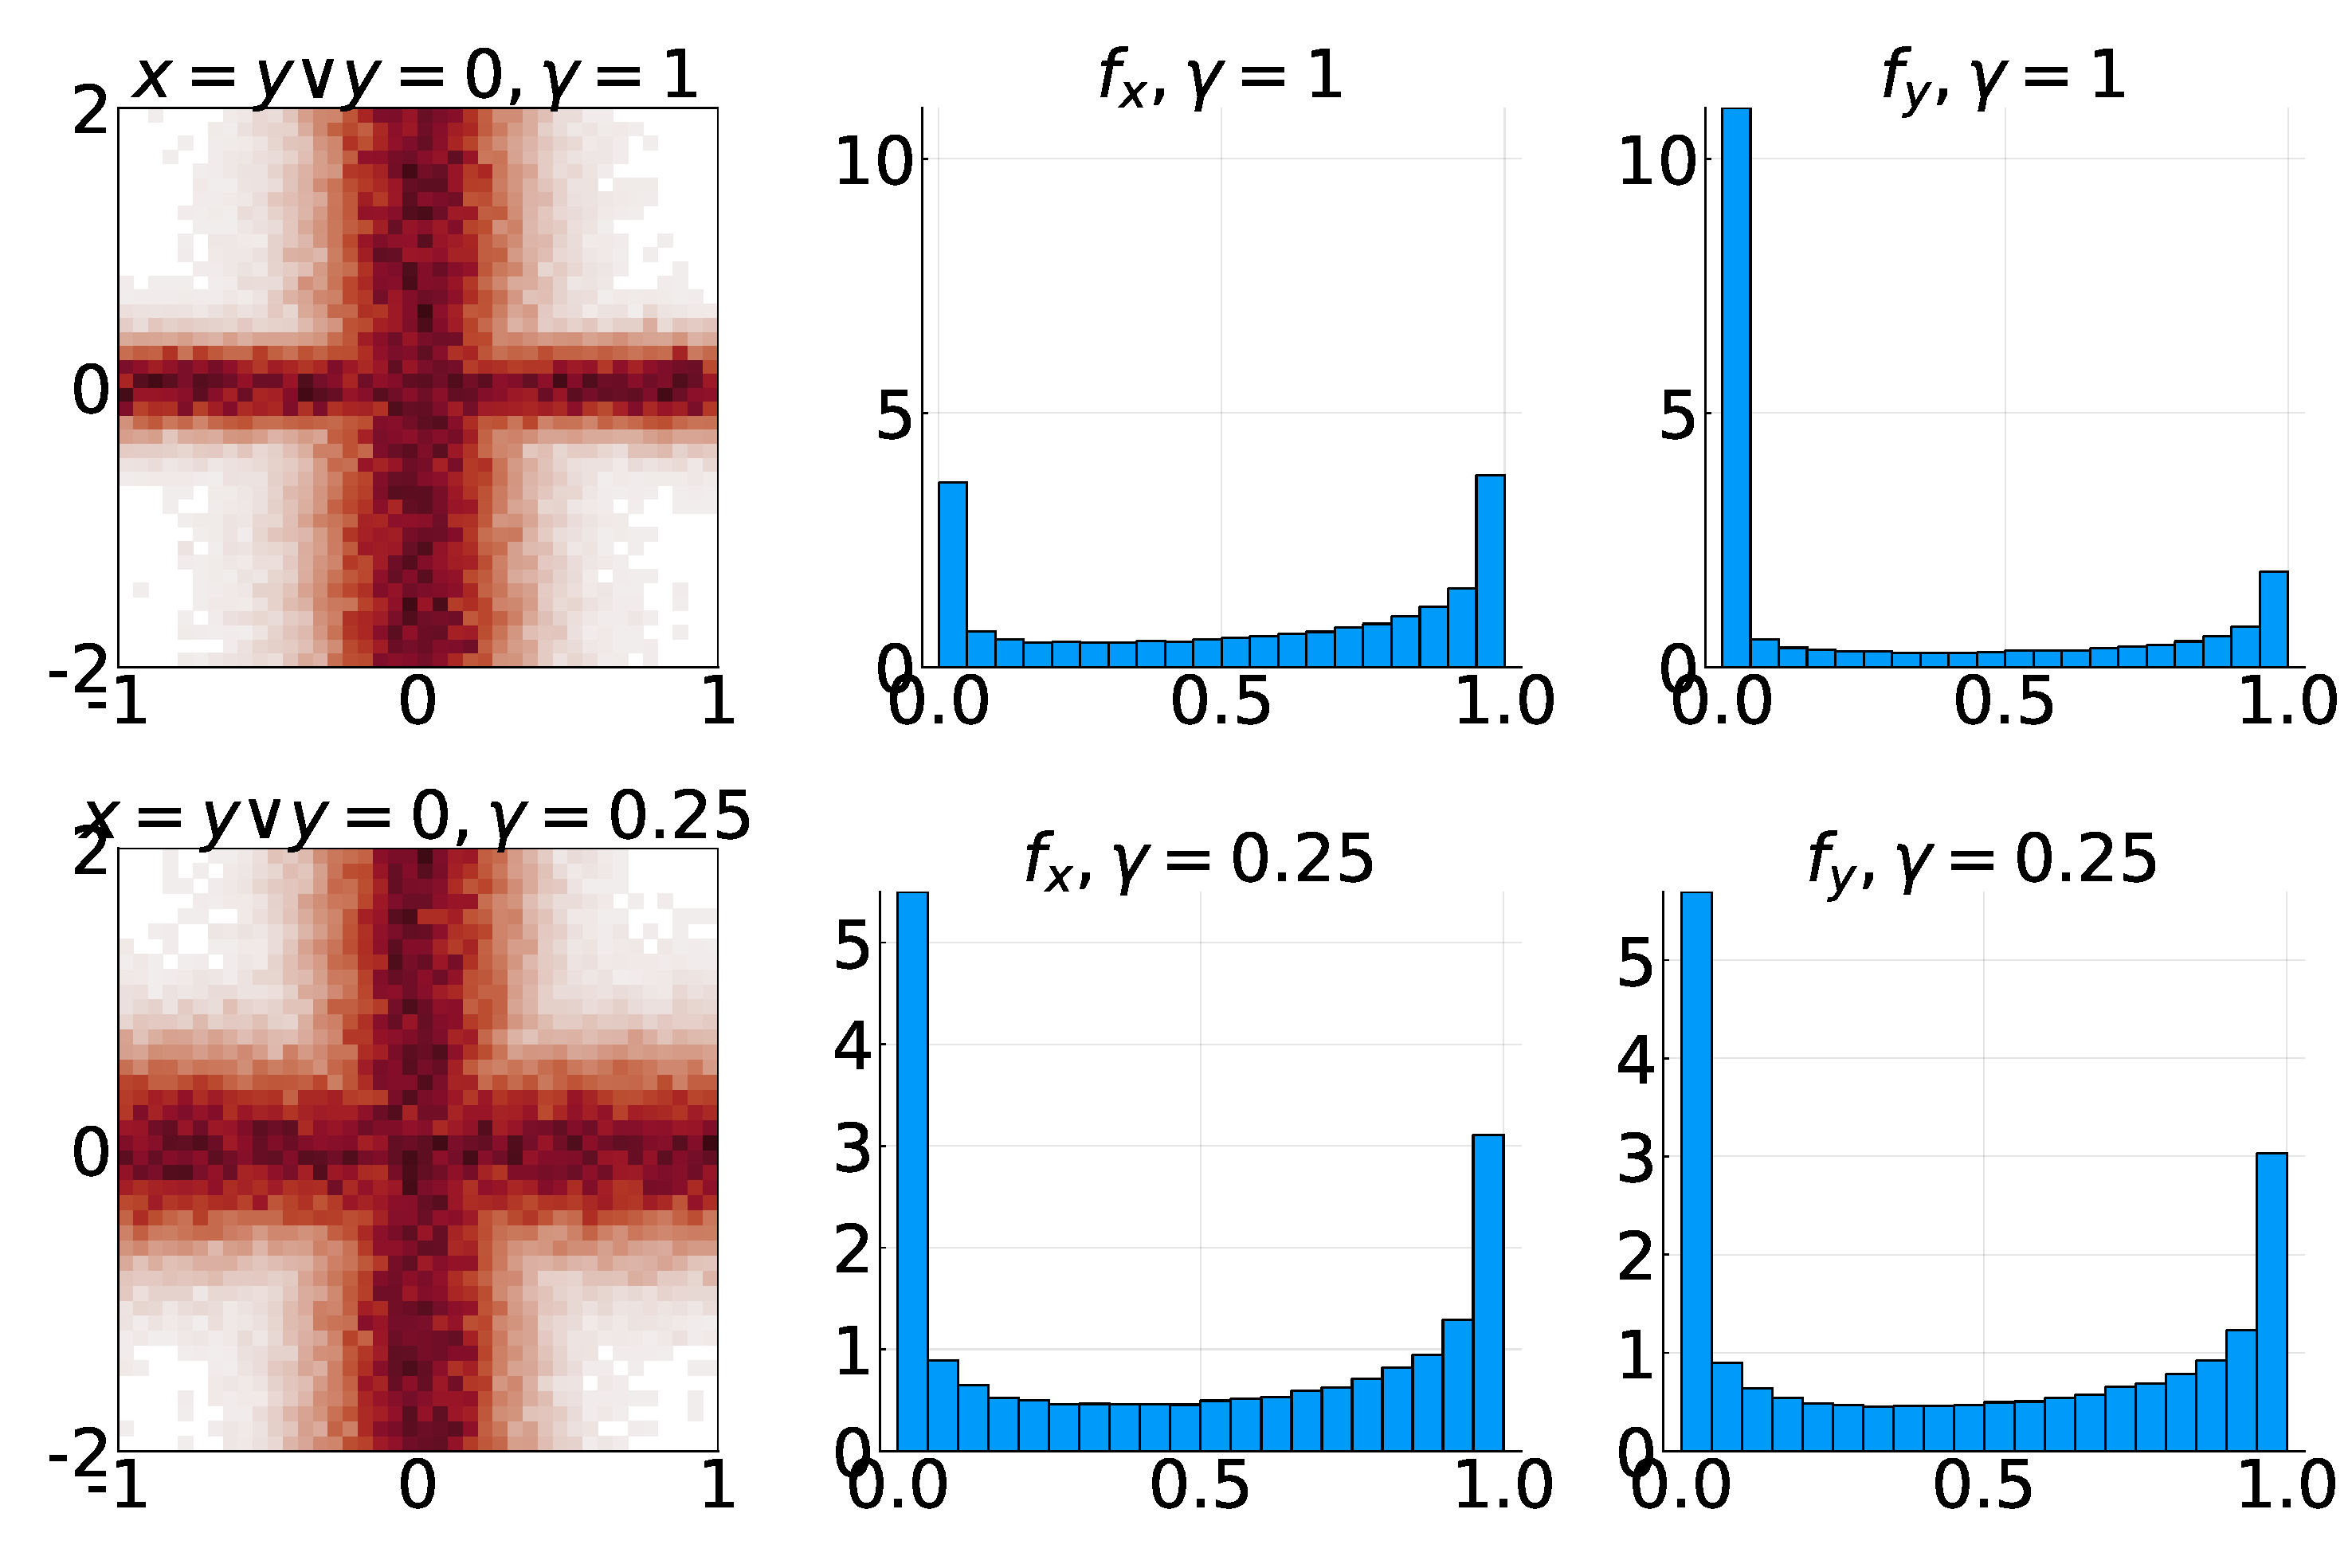
\includegraphics[width=0.9\linewidth]{scaling.pdf}
  \caption{Scaling Properties.}\label{scaling}
  \end{figure}

  
\subsection{Replica Exchange}\label{replicaexchange}
Replica exchange \citep{swendsen1986replica} simulates $M$ replicas of a model at different temperatures, and uses a Metropolis-Hastings update to  periodically swap the temperatures of chains.
Let $f_{\alpha_i}$ denote the approximate posterior function at temperature $\alpha_i$, then two independent parallel chains simulating targets $f_{\alpha_1}(x)$, $f_{\alpha_2}(y)$  follow a joint target $f_{\alpha_1, \alpha_2}(x,y) = f_{\alpha_1}(x)f_{\alpha_2}(y)$.
Replica exchange swaps states between the chains while preserving the joint target.
Swapping states is equivalent to swapping predicates, which motivates the name ``predicate exchange''.
Concretely, replica exchange proposes a swap from $(x, y)$ to $(y, x)$, and accepts it with probability $\min(1, A)$, where:
\begin{equation}
A =  \frac{f_{\alpha_1, \alpha_2}(y,x)}{f_{\alpha_1, \alpha_2}(x,y)} = \frac{f_{\alpha_1}(y)f_{\alpha_2}(x)}{f_{\alpha_1}(x)f_{\alpha_2}(y)}
\end{equation}

We modify standard replica exchange in two ways: (i) for exact inference, states which violate the constraint are rejected, and (ii)
unlike conventional replica exchange which draws samples only from the zero-temperature chain, we accept states from any chain so long as $f_{\alpha_i}(x) = 1$.


% \paragraph{Unsatisfiability}Predicate exchange is unable to determine if a predicate is unsatisfiable (e.g.  $(x > 1) \land (x < -1)$), and defers to the user to ensure this is not the case.




% This scenario closely resembles the reparameterization trick \citep{Kingma:2014, rezende2014stochastic} where one resorts to include all the uncertainty of a random variable $z$ in a simple, easy-to-sample, parameter-free noise source such as $\epsilon \sim \mathcal{N}(\mathbf{0}, I)$. The actual random variable $z$ is then obtained through a parametric transformation of the noise, $z = f(\epsilon; \theta)$. Both methods separate the 
% uncertainty of a random variable from the deterministic transformation that results in a complex density. However, in the reparameterization trick the noise source is constant and controlled while the parametric transformation is meant to infer the structure of the resulting random variable. Conversely, our forward model -- deterministic transformation -- is constant and controlled, hence we simply transfer our inference problem to a much simpler space of $\Omega$.

% Predicate Exchange has a connection to approximate Bayesian computation (ABC) methods~\citep{beaumont2002approximate} in that ABC methods 
% sample using a distance function to induce a data likelihood. Our method differs in that conditionals can be any predicate not just
% one for an observed random variable.
% Finally for inference, with the soft predicates we define, we
% can use modern likelihood-free variational inference algorithms
% that construct an approximation to a conditional with only samples
% from the joint and samples from the conditional approximation~\citep{tran2017hierarchical}.

